\chapter{Preliminary Work}
\label{chap:prelim_work}

%--------------------------------------------------------------------------------------------------------------------------------------------------------------------
%--------------------------------------------------------------------------------------------------------------------------------------------------------------------
%--------------------------------------------------------------------------------------------------------------------------------------------------------------------
%--------------------------------------------------------------------------------------------------------------------------------------------------------------------
%--------------------------------------------------------------------------------------------------------------------------------------------------------------------
%--------------------------------------------------------------------------------------------------------------------------------------------------------------------
%--------------------------------------------------------------------------------------------------------------------------------------------------------------------
\section{Nonlinear \cobra}
\label{sect:nl_cobra}
The first stage of preliminary work was to modify the \cobra software.
\cobra 
When it is necessary to distinguish between the single-shot linearization algorithm of \cobra and the iterative nonlinear algorithm of\cobra, the former shall be referred to as legacy mode and the latter as nonlinear mode.

%--------------------------------------------------------------------------------------------------------------------------------------------------------------------
%--------------------------------------------------------------------------------------------------------------------------------------------------------------------
%--------------------------------------------------------------------------------------------------------------------------------------------------------------------
%--------------------------------------------------------------------------------------------------------------------------------------------------------------------
%--------------------------------------------------------------------------------------------------------------------------------------------------------------------
%--------------------------------------------------------------------------------------------------------------------------------------------------------------------
%--------------------------------------------------------------------------------------------------------------------------------------------------------------------
\section{Temporal Convergence}
\label{sect:temporal_convergence}
The question of temporal convergence is linked not only to the particular method used for approximating the temporal derivatives, but also to the degree to which the nonlinearities are resolved over a time-step. 

%--------------------------------------------------------------------------------------------------------------------------------------------------------------------
%--------------------------------------------------------------------------------------------------------------------------------------------------------------------
%--------------------------------------------------------------------------------------------------------------------------------------------------------------------
%--------------------------------------------------------------------------------------------------------------------------------------------------------------------
%--------------------------------------------------------------------------------------------------------------------------------------------------------------------
%--------------------------------------------------------------------------------------------------------------------------------------------------------------------
%--------------------------------------------------------------------------------------------------------------------------------------------------------------------

\section{Operator Based Scaling}
\label{sect:operator_scaling}
In order to determine the degree to which a state vector, $\vec{x}$, satisfies \eqref{eqn:conservation_equations}, the use of the nonlinear residual, $\vec{F}$, is required.
However, due to the formulation of the residual vector, the magnitudes of residuals can vary by orders of magnitude.
For a given grid location, the nonlinear residuals for mass and energy, \eqref{eqn:cont_residual}, as formulated in section \ref{subsect:semi_implicit} will have six components.
These residuals will have the units of the conserved quantities for their corresponding PDEs.
Table \ref{tab:scaling_units_scales} shows some typical values of these conserved quantities during normal operations of typical PWR simulation.

\begin{table}[ht]
\centering
\begin{tabular}{@{}lr@{.}lr@{.}lr@{.}lr@{.}lr@{.}l@{}} \toprule
\multirow{2}{*}{Problem} & \multicolumn{2}{c}{Pressure} & \multicolumn{2}{c}{Enthalpy}             & \multicolumn{2}{c}{$\alpha_g$} & \multicolumn{2}{c}{$\alpha_l$} & \multicolumn{2}{c}{$\alpha_e$} \\ 
                         & \multicolumn{2}{c}{[psia]} & \multicolumn{2}{c}{$[\frac{\text{Btu}}{\text{lb}_{\text{m}}}]$} & \multicolumn{2}{c}{[-]}      & \multicolumn{2}{c}{[-]}      & \multicolumn{2}{c}{[-]}      \\ \midrule
Single Phase             &  200&0                       &  355&5                                   & 0&0                            & 1&0                            & 0&0 \\
Flashing                 &  200&0                       & 1198&3                                   & 1&0                            & 0&0                            & 0&0 \\ \bottomrule  
\end{tabular}
\caption{Typical scale for reactor simulations}
\label{tab:scaling_units_scales}
\end{table}

However, during accident scenarios, the range of these values can dramatically change.
One of the challenges that has been addressed during this work is coming up with a method for scaling that will provide a meaningful metric for convergence.
The scaling chosen should have the following characteristics:
\begin{itemize}
\item{$S^{-1}_k F(x_k)_i \approx 1$ when $x_k$ is a "poor" solution.}
\item{$S^{-1}_k F(x_k)_i \rightarrow 0$ when a phase disappears.}
\item{$0 \leq S^{-1}_k F(x_k)_i \leq 0 $ for all values of $F(x_k)_i$.}
\end{itemize}

The heart of the scaling used in this work is a physics-based method.
To illustrate the scaling procedure, we shall consider \eqref{eqn:conservation_of_liq} for a simply connected continuity cell without inter-field mass transfer.
Assume that the entire channel single phase and in thermodynamics equilibrium such that the macroscopic densities on either side of this single cell are the same.

\begin{equation}
F = \left(\alpha_k \rho_k\right)^{n+1} - \left( \alpha_k \rho_k \right)^n - \frac{\Delta t}{V} \left( \frac{\alpha_k \rho_k }{<\alpha_k \rho_k>^n} V^{n+1}_{j-1} \right)
\end{equation}

In this equation there are three physically meaningful quantities: the temporal difference, the mass flowing into the cell, and mass flowing out of the volume.
%--------------------------------------------------------------------------------------------------------------------------------------------------------------------
%--------------------------------------------------------------------------------------------------------------------------------------------------------------------
%--------------------------------------------------------------------------------------------------------------------------------------------------------------------
%--------------------------------------------------------------------------------------------------------------------------------------------------------------------
%--------------------------------------------------------------------------------------------------------------------------------------------------------------------
%--------------------------------------------------------------------------------------------------------------------------------------------------------------------
%--------------------------------------------------------------------------------------------------------------------------------------------------------------------

\section{Numerical Experiments}
\label{sect:numerical_experiments}

Two test problems were constructed to examine the impact of nonlinear convergence on temporal convergence.
The primary purpose of the problems studied is to determine the impact of resolving the nonlinearities at each time step for a given time-step size on the number of time-step size refinements necessary to reach a temporally converged solution.

\subsection{Geometry}
\label{subsect:experimental_geometry}
For both of the test problems, the same computational geometry was used; figure \ref{fig:exp_geometry} represents the experimental geometry.
Each block represents a single continuity cell with a height of 4 [in].
The total height of the channel is 48 [in].
Each continuity cell has a cross-sectional area of 4 [in$^2$] and a hydraulic diameter of 4 [in].
The red block at the top of the channel represents a boundary cell where the pressure and enthalpy are specified.
This boundary represents an infinite reservoir filled with a fluid at a specified thermodynamic state.
The red triangle represents a specified flow at the bottom edge of the first continuity cell. 
\begin{figure}[h!t]
\caption{Geometry for test problems.}
\label{fig:exp_geometry}
\begin{center}
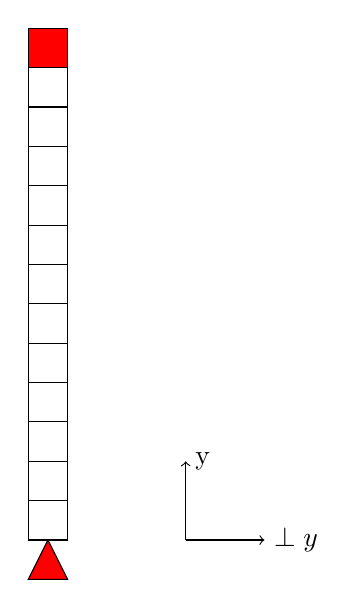
\begin{tikzpicture}
\foreach \x in {1,..., 12} \draw(0, 0.5*\x-0.5) rectangle +(.5,.5);
\filldraw[fill=red] (0, 6) rectangle +(.5,.5); 
\filldraw[fill=red] (0, -0.5) -- (0.25, 0) -- (0.5, -0.5) -- cycle;
\draw[->] (2,0) -- (2, 1) node[anchor=west] {y};
\draw[->] (2,0) -- (3, 0) node[anchor=west] {$\perp y$};
\end{tikzpicture}
\end{center}
\end{figure}

\subsection{Initial and Boundary Conditions}
\label{subsect:ic_bc}

The two problems, while having the same geometry, are different in their dominant physics.
One problem was designed to represent single-phase, single-field continuous liquid flow in a standpipe; this problem will be referred to as the "Single Phase" problem.
The second problem was designed such that high pressure liquid flashes into steam as it enters a standpipe initially filled with saturated vapor at a much lower pressure, known hereafter as the "Flashing" problem.

Table \ref{tab:ic} provides the initial conditions for the two problems.
The pressure, enthalpy, and volume-fractions for the different fields allows for a complete description of the continuity variables.
The initial velocities are set to zero.

\begin{table}[h!t]
\centering
\begin{tabular}{@{}lr@{.}lr@{.}lr@{.}lr@{.}lr@{.}l@{}} \toprule
\multirow{2}{*}{Problem} & \multicolumn{2}{c}{Pressure} & \multicolumn{2}{c}{Enthalpy}             & \multicolumn{2}{c}{$\alpha_g$} & \multicolumn{2}{c}{$\alpha_l$} & \multicolumn{2}{c}{$\alpha_e$} \\ 
                         & \multicolumn{2}{c}{[psia]} & \multicolumn{2}{c}{$[\frac{\text{Btu}}{\text{lb}_{\text{m}}}]$} & \multicolumn{2}{c}{[-]}      & \multicolumn{2}{c}{[-]}      & \multicolumn{2}{c}{[-]}      \\ \midrule
Single Phase             &  200&0                       &  355&5                                   & 0&0                            & 1&0                            & 0&0 \\
Flashing                 &  200&0                       & 1198&3                                   & 1&0                            & 0&0                            & 0&0 \\ \bottomrule  
\end{tabular}
\caption{Initial conditions for test problems.}
\label{tab:ic}
\end{table}

Each of the problems has a specified pressure-enthalpy boundary condition at the top of the stand pipe and a flow-enthalpy boundary condition at the inlet of the domain.
Table \ref{tab:bc_pe} contains the pressure, enthalpy, and composition of the pressure-enthalpy resevior. 

\begin{table}[h!t]
\centering
\begin{tabular}{@{}lr@{.}lr@{.}lr@{.}lr@{.}lr@{.}l@{}} \toprule
\multirow{2}{*}{Problem} & \multicolumn{2}{c}{Pressure} & \multicolumn{2}{c}{Enthalpy}             & \multicolumn{2}{c}{$\alpha_g$} & \multicolumn{2}{c}{$\alpha_l$} & \multicolumn{2}{c}{$\alpha_e$} \\ 
                         & \multicolumn{2}{c}{[psia]} & \multicolumn{2}{c}{$[\frac{\text{Btu}}{\text{lb}_{\text{m}}}]$} & \multicolumn{2}{c}{[-]}      & \multicolumn{2}{c}{[-]}      & \multicolumn{2}{c}{[-]}      \\ \midrule
Single Phase             &  200&0                       &  355&5                                   & 0&0                            & 1&0                            & 0&0 \\
Flashing                 &  200&0                       & 1198&3                                   & 1&0                            & 0&0                            & 0&0 \\ \bottomrule  
\end{tabular}
\caption{Pressure-enthalpy boundary conditions for test problems.}
\label{tab:bc_pe}
\end{table}

The flow-enthalpy boundary condition describes the thermodynamic state of the inflowing fluid and the rate at its flowrate.
Table \ref{tab:bc_fe} describes the inlet boundary condition for the two problems.

\begin{table}[h!t]
\centering
\begin{tabular}{@{}lr@{.}lr@{.}lr@{.}lr@{.}lr@{.}l@{}} \toprule
\multirow{2}{*}{Problem} & \multicolumn{2}{c}{Pressure} & \multicolumn{2}{c}{Enthalpy}             & \multicolumn{2}{c}{$\alpha_g$} & \multicolumn{2}{c}{$\alpha_l$} & \multicolumn{2}{c}{$\alpha_e$} \\ 
                         & \multicolumn{2}{c}{[psia]} & \multicolumn{2}{c}{$[\frac{\text{Btu}}{\text{lb}_{\text{m}}}]$} & \multicolumn{2}{c}{[-]}      & \multicolumn{2}{c}{[-]}      & \multicolumn{2}{c}{[-]}      \\ \midrule
Single Phase             &  200&0                       &  355&5                                   & 0&0                            & 1&0                            & 0&0 \\
Flashing                 & 1000&0                       &  542&6                                   & 1&0                            & 0&0                            & 0&0 \\ \bottomrule  
\end{tabular}
\caption{Flow-enthalpy boundary conditions for test problems.}
\label{tab:bc_fe}
\end{table}

The specified mass flow, $\dot{m}(t)$, at the bottom of the channels is the same for both problems. 
The is a time-dependent function give by \eqref{eqn:bc_time_func_single}.

\begin{equation}
\label{eqn:bc_time_func_single}
\dot{m}(t) = \left\{
\begin{array}{cclrcll}
 0.0           & [\frac{\text{lb}_{\text{m}}}{\text{s}}] & , &         & t & \leq 1 &[\text{s}] \\
 0.5 ( t - 1)  & [\frac{\text{lb}_{\text{m}}}{\text{s}}] & , & 1 [\text{s}] < & t & \leq 2 &[\text{s}] \\
 0.5           & [\frac{\text{lb}_{\text{m}}}{\text{s}}] & , &         & t & > 2    &[\text{s}]
\end{array}\right.
\end{equation}

Both problems adjust their initial pressure distribution to account for hydrostatic head, which is not specified on the inlet cards.
The COBRA-IE input deck for both problems can be found in \app{app:input_decks}.

\subsection{Procedure}
\label{subsect:experiments_procedure}
To determine the effect of nonlinear convergence upon the time-step size sensitivity of the solution, each problem was run for at increasingly small maximum $\Delta t$.
The material CFL limit of semi-implicit method acted as a limiter on the time-step size selected.
If the acceptable time-step size was below

\subsection{Results}
\label{subsect:results}


\section{Review}
\label{sect:review}

